
\documentclass[a4paper, 12pt]{article}
\usepackage[top=3cm, bottom=3cm, left = 2cm, right = 2cm]{geometry} 
\geometry{a4paper} 
\usepackage[utf8]{inputenc}
\usepackage{textcomp}
\usepackage{graphicx} 
\usepackage{amsmath,amssymb}  
\usepackage{bm}  
\usepackage[pdftex,bookmarks,colorlinks,breaklinks]{hyperref}  
\hypersetup{linkcolor=black,citecolor=black,filecolor=black,urlcolor=black} % black links, for printed output
\usepackage{memhfixc} 
\usepackage{pdfsync}  
\usepackage{fancyhdr}
\usepackage{enumitem}
\usepackage{cite}
\usepackage{txfonts}
\usepackage{setspace}
\usepackage{siunitx}
\usepackage{lipsum}
\usepackage{natbib}
\usepackage{eucal}
\usepackage{physics}
\usepackage{cancel}
\usepackage[autostyle]{csquotes}
\newcommand{\tn}[1]{\textnormal{#1}}
\graphicspath{{./images}}

\title{Appearance of Quasinormal modes in Quantum Gravity \\
        \large Project report\\}
\author{Yamamoto Sho}


%\date{}
\begin{document}
\maketitle
\tableofcontents

\section{Abstract}
  Quasinormal modes (QNMs) refer to the eigenmodes of dissipative harmonic
  oscillators. These modes appear canonically when studying
  gravitational waves (GWs) generated by black holes (BHs). In
  this paper, we review the appearance of QNMs in various quantum gravity
  (QG), namely AdS/CFT correspondence in string theory, and the Immirzi
  parameter in loop quantum
  gravity (LQG).
\section{Introduction}

In a typical BH-BH merger event, the ringdown, which is referred to as the event
from which the two BHs merged into one the merged BH settled down from
the perturbation due to the collision forms a stable non-oscillating
BH. It is this ringdown that produces a QNM signal, which is
characterized by a complex frequency $ \omega \in \mathbb{C} $.  

QNMs serve a wide variety of uses in studying modern physics, with constraining
modified gravity and QG being the prominent research
direction\cite{volkel2022constraining}\cite{gogoi2024constraints}. 
This review paper begins by briefly introducing the physical picture
of string theory, namely the AdS/CFT correspondence, and the Immirzi
parameter appearing in quantized
area in LQG, see (\ref{sec:Background}) Followed by the precise description in which QNMs appear in
the two aforementioned theories, see section (\ref{sec:Appearance of QNMs in QG}),
and concluding with the promising future direction for theoretical
research in QG through studying QNMs. 














\section{Background}



 


\subsubsection{AdS/CFT correspondence}

In this section, we review the concept of AdS/CFT correspondence, in
particular, we briefly give insights to the correspondence with Maldacena's
case\cite{maldacena1999large} while omitting some details, in particular
the consideration of supersymmetry (SUSY) that goes into the
correspondence. For a review of SUSY, one may refer to
\cite{sohnius1985introducing}. 

It is also beneficial to rephrase the correspondence in detail. It states
that, in Maldacena's study

\begin{align}
  \label{maldacena case}
  \begin{split}
\textnormal{Type IIB string theory on 
  }\mathrm{AdS}_5 \times S^5 &\equiv 4D  \textnormal{  super-Yang-Mills
  (SYM) theory, with} \\
  \textnormal{(or the low energy limit supergravity)}  & \hspace{0.5cm}\mathcal{N} = 4 \textnormal{ SUSY, and gauge group SU(N).
 } 
  \end{split}
\end{align} The equivalence here means in particular that in the end we have
the relationship 
\begin{align}
  \label{ads cft equivalence}
  Z_{4D}[J] \equiv \int \dd[]{\phi} e^{iS + \int i \dd[4]{x}J \mathcal{O}}
  = e^{i S_{cl}},  
\end{align}with \( Z_{4D} \) denoting the partition (or generating)
function of the \textnormal{R.H.S.} of (\ref{maldacena case}), while \(
S_{cl} \) denoting the classical action on the \textnormal{L.H.S.}. 

\subsubsection{The CFT side of Maldacena's case}
 \label{cft side} 
  The CFT side, i.e. \textnormal{R.H.S.} of (\ref{maldacena case}),
  while neglecting SUSY, can be interpreted simply as the SU(N) YM 
  theory in 4-dimensional space, in particular, N = 3 is the
  familiar Quantum Chromodynamics (QCD). The physical
  interpretation for this is thus as intuitive as a theory describing
  N-color charged particles. 

  It is also worth mentioning one general feature of SU(N) YM theories
  are non-perturbative. In particular, QCD is indeed
  non-perturbative, and that the dual AdS side is otherwise, which
  motivates for more study into the correspondence, as it can give more
  insight into non-perturbative QFT. 

\subsubsection{The AdS side of Maldacena's case} 
\label{ads side}
  The AdS side, i.e. \textnormal{L.H.S.} of (\ref{maldacena}), is
  essentially type IIB string theory on \( \mathrm{AdS}_5 \cross S^{5}  \).
  some tricks considered by Maldacena, one may in fact
  physically interpret this as gravity in 5D, which again the SUSY is
  ignored for providing physical intuition. 

  To demonstrate it mathematically, we begin by considering N coincident
  D3-brane on type IIB string
  theory on \( \mathrm{AdS}_5 \cross S^{5}  \) and in Maldacena's case, the
  branes are placed at the origin, and encoded hidden in the extra
  dimensions that are not visible to us. It is then possible
  to obtain the solution for this system, with equations for the D-branes,
  and with the solution of the spacetime metric as
     \begin{align}
       \label{ads metric}
        \mathrm{d}s^2 &= \bigg( 1 + \frac{L^4}{y^4}  \bigg)^{-1/2}
     \eta_{ij} \mathrm{d}x^i \mathrm{d}x^j  + \bigg( 1 + \frac{L^4}{y^4}
       \bigg)^{1/2}(\mathrm{d}y^2
       + y^2 \mathrm{d}\Omega_5^2),
     \end{align} where L is the radius of the D3-brane, with the
     relation \( L^4 = 4 \pi g_s N(\alpha^{\prime})^2 \), while \(
     x^{i}, y^{\mu}   \) denote the coordinates both parallel and
     perpendicular to the brane respectively. To have a better
     understanding this geometry, we first make the change of
     variable \( u \equiv L^2/y  \), and take the limit \( u \to \infty
     \), resulting 
     \begin{align}
      \label{ads better metric}
        \mathrm{d}s^2 = L^2 \bigg( \frac{1}{u^2} \eta_{ij}
        \mathrm{d}x^i \mathrm{d}x^j  + \frac{\mathrm{d}u^2}{u^2}
        + \mathrm{d}\Omega_{5}^{2}\bigg).
    \end{align} First, the interpretation of this limit is simply zooming
    into the brane, and the first two terms
    correspond to the geometry \( \mathrm{AdS}_5 \) as \( \eta_{ij}
    = \mathrm{diag}(-1, 1, 1, 1)\). The latter term \(
    \mathrm{d}\Omega_{5}^{2} \) denotes the 5-sphere and thus the geometry
    \( S^5 \) that are hidden to us. 
    \begin{figure}[h!]
    \begin{center}
      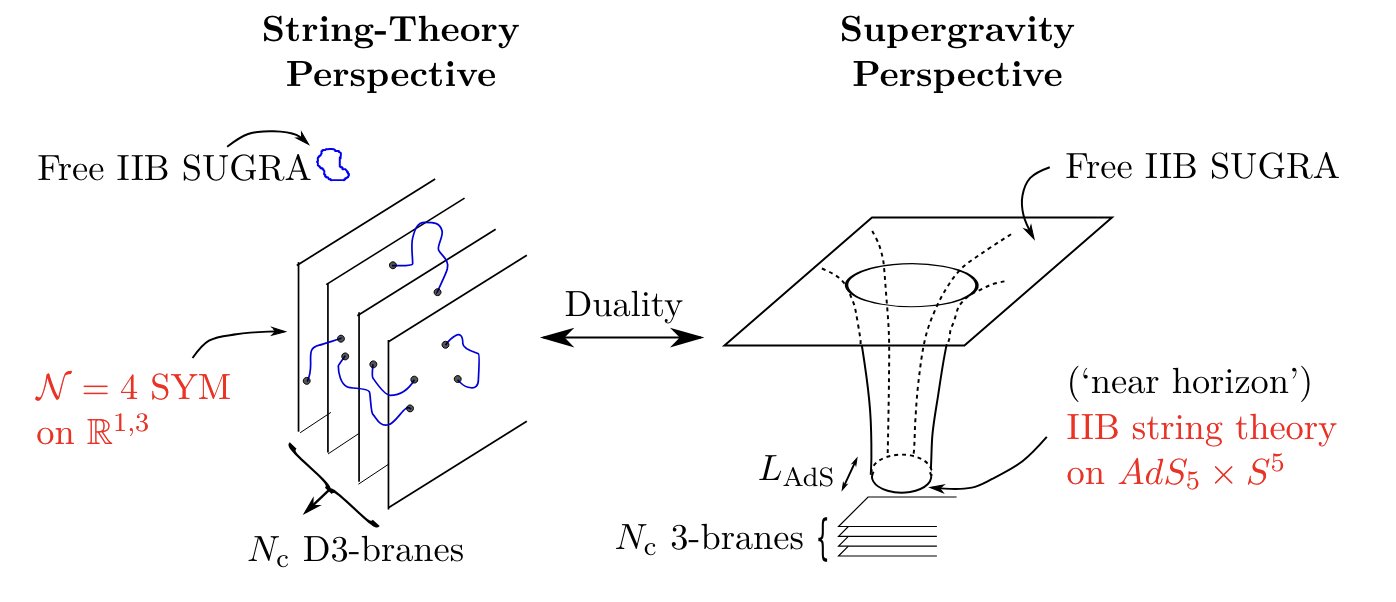
\includegraphics[scale=0.4]{Figures/duality.png}
    \end{center}
    \caption{Sketch of the AdS/CFT duality. On the CFT side, it is the
      \(\mathcal{N}\) = 4 SYM, or interpreted in string theory as D-3
      branes stack that produce the SYM gauge fields. On the other
      hand, it is the low-energy limit SUGRA perspective, where the
      spacetime metric of the form \( \mathrm{AdS}_5 \times S^5 \)
      that is dual to the other. Modified from
      \cite{samberg2012holographic}.}
    \label{fig:duality}
    \end{figure}

  \subsubsection{Maldacena's correspondence}%
    \label{sub:Maldacena's correspondence}
   The Maldacena's correspondence states that if we identify the
   coupling constants of the two theories discussed previously, namely \(
   g_{\mathrm{YM}}^{2} = 4 \pi g_{s}, \hspace{0.5cm} g_{YM}^{2} N_c = L^2
   / \alpha^{\prime}\), where \( \alpha^{\prime} \) is the universal
   Regge slope, \( g_s, N_c, \textnormal{ and } g_{\mathrm{YM}} \) string coupling
   constant, number of colour charges and YM coupling constant, Maldacena
   showed that
   \begin{align}
    \label{correspondence}
     Z_{\mathrm{CFT}}[J] \equiv e^{i S_{cl}}.  
   \end{align} In other words, the generating function of the CFT side is
   equivalent to the exponent of the action of the dual AdS gravity
   theory. This remarkable result motivated others to look for more such
   correspondences in different settings. Later t'Hooft
   conjectured, motivated by the holographic
   principle\cite{susskind1995world}, that any D+1 dimensional gravity
   is dual to its D dimensional CFT\cite{hooft2001holographic}. 
   
   \subsection{Loop Quantum Gravity and Immirzi parameter}  
   \label{sub:Loop Quantum Gravity and Immirzi parameter}
    LQG is a candidate for QG, with its formalism based on 3+1
    decomposition, or so-called ADM formalism, of general
    relativity(GR)\cite{corichi2022introduction}. It was
    Ashtekar\cite{ashtekar2021short} further
    had the inspiration to decompose the spatial metric as
    composition of two densitized triad
    \begin{align}
      \label{spatial metric lqg}
      \tilde{E}_{i}^{a} &= \sqrt{\mathrm{det}(h)} E_{i}^{a},
    \end{align} with this and the spatial metric related by \(
    \mathrm{det}(q) q^{ab} = \tilde{E}_{i}^{a} \tilde{E}_{j}^{b}
    \delta_{}^{ij} \), where the indices (a,b) denote the spin once the
    spin \textit{connection} is defined from this theory which is
    constructed similarly to the Christoeffel connection for GR. 

    Proceeding quantization under this formalism, the
    quantized area 
    of this theory can be obtained, which is given by 
    \begin{align}
      \label{area operator}
      A(j) &= 8 \pi l_{P}^{2} \gamma \sqrt{j(j+1)},    
    \end{align} where \( l_P \) is the Planck length and \( \gamma \)
    the Immirzi parameter, while the positive half-integers \( j \)
    denotes the spin representation of the given
    surface\cite{ashtekar1997quantum}. 
    

  \section{Appearance of QNMs in QG}%
    \label{sec:Appearance of QNMs in QG}
    In this section, we mention the appearance of QNMs in certain QG
    theories, namely string theory and LQG.  


    \subsection{Appearance of QNMs in string theory}%
      \label{sub:Appearance of QNMs in string theory}
      

    It was shown by Birmingham, Sach and Solodukhin that for 
    the AdS/CFT correspondence, with \( \mathrm{AdS}_{2+1} \)
    at the near-horizon geometry as the AdS side dual to the
    corresponding CFT, the QNMs of the gravity side is exactly the
    poles of the retarded correlation function of the dual CFT\cite{birmingham2002conformal}. 

    The QNMs in this setting, with the Banados-Teitelboim-Zanelli
    (BTZ) BH
    as the metric solution\cite{karakasis2021black}, we obtain 
    \begin{align}
      \label{QNM in (2+1)}
      \omega &= \pm k - 4 \pi T i (n + 1), 
    \end{align} where k denotes momentum, T the Hawking
    the temperature of BTZ BH and n the modes. 

    There are more on-going search for the appearance of QNMs in
    different AdS/CFT settings, and it is also possible that one can
    constraint the string landscape with observational QNMs through
    AdS/CFT correspondence of 4D gravity dual to 3D CFT. 

    \section{Role of QNMs in LQG}%
      \label{sec:Appearance of QNMs in LQG}
   
    Rather than QNMs appearing LQG, QNMs provide a way to fix Immirzi
    parameter in the theory, given there are no conclusive ways to obtain
    a consistent Immirzi parameter theoretically. To do so, we may
    refer to numerical result of QNMs, and match it with the
    theory\cite{dreyer2003quasinormal}.

    For example, taking the result from
    Nollert\cite{nollert1999quasinormal}, we have the numerical QNM
    value as 
    \begin{align}
      \label{QNM nollert}
      M \omega = 0.04371235 + \frac{i}{4}(n + \frac{1}{2}), 
    \end{align} where M is the mass of the merged BH, this result was
    later observed that the constant real part is equal to \(
    \mathrm{ln}3 / 8\pi \).  
    
    We can then fix the Immirzi parameter by computing the entire surface
    of the BH through the (\ref{area operator}), with the surface of the
    Schwarzschild BH related to M by \( A = 16 \pi M^2 \). With these systems
    of equations, and consideration of the Bekenstei-Hawking
    equation, in turn then fixes the Immirzi parameter as 
    \begin{align}
      \label{immirzi fixed}
      \gamma = \frac{\mathrm{ln}3}{2 \pi \sqrt{2} }.
    \end{align}

   \section{Conclusion}%
    \label{sec:Conclusion}
    To conclude, QNMs are closely related to QG as naturally the dynamics
    of QNMs are encoded by the dynamics of BHs, which requires QG to fully
    describe its nature. We have reviewed where this is observed in the
    theory, namely QNMs are related to the poles in the retarded green
    the function of the CFT theory that is dual to the QNMs generated
    by the BH solution in the AdS gravity via the
    AdS/CFT correspondence. However, we still lack enough research
    on more cases to validate and generalise this observation in the
    theory. We also reviewed the numerical results of QNM serve to fix
    the Immirzi parameter in LQG, though once again more
    verifications are needed to justify the procedure, as there could be
    degeneracies from both the theory and the numerical results. 


  





\newpage
\bibliographystyle{unsrt}
\bibliography{references.bib}
        
\end{document}

